\chapter{使用 \headinglatin{\ksonline}}\label{ch:online}
\index{Zaixian ban@在线版}

\ksonline{} 将工具箱工作区放在浏览器中，无须在本机安装客户端。结构编辑、工作流与结果分析仍在主窗口中进行，实际运算由服务器完成。瀚海量子\regmark{}官方在线版即将推出，并支持集群私有化部署。通过所选部署提供的入口登录账号后，便可进入分配的工作空间。

在线版与桌面应用最需要区分的地方是文件和会话。本机文件需要上传，项目通常保存在云端“文件”面板中，下载后才得到个人计算机上的副本。关闭网页、返回入口和注销也有不同含义。本章通过一个硅结构项目，把这些操作串成一次完整的练习。

\section{进入自己的工作空间}

\subsection{开始前准备什么}

准备好所选部署提供的在线地址、可用账号，以及随书的小型结构文件。首次注册可能需要邀请码，按部署页面给出的注册方式操作。浏览器应能正常运行 WebGL，以便显示三维原子结构。

尽量使用较大的浏览器窗口。窗口较小时，中央视图与参数编辑区会同时变窄，长表单可能需要滚动。在笔记本上可以先收起暂时不用的侧边面板；这样仍能保留工具栏和正在编辑的文档。

同一个工作空间保持一个活动浏览器标签页即可。如果已经在另一标签页打开工作区，应先返回原标签页继续使用，或关闭旧连接后再连接。不要用多个标签页反复尝试抢占同一工作空间。

\subsection{注册账号}

固定入口首先显示登录页。需要新账号时，切换到注册页，按表单依次填写。账号名使用小写字母、数字或连字符，以字母开头，长度为 3--32 个字符；密码长度为 12--128 个字符，并需再次输入确认。

注册还需要备忘问题、备忘答案和邀请码。问题会用于找回密码，应选择自己能记住的问题；答案则应是自己能记住、他人不易猜到的内容。不要把密码写进备忘问题。问题和答案填写后，点击 \ui{注册账号}，成功后返回登录页。

% SCREENSHOT: 真实在线版登录与注册页，所有账号输入保持空白；突出两个页面的用途差异。

\subsection{登录并等待启动}

\begin{steps}
\item 在固定入口的登录页填写个人账号信息。
\item 点击 \ui{登录并打开工作空间}。
\item 等待入口显示工作空间准备状态。第一次启动可能比以后更久。
\item 工作空间就绪后进入工具箱主界面；如果入口显示 \ui{打开工作空间}，点击该按钮继续。
\item 确认上方出现工具栏，左侧可打开\ui{项目浏览器}和\ui{文件}面板，中央文档区能够响应操作。
\end{steps}

入口可能显示“正在启动”“已就绪”等状态。状态变化时保持页面打开即可，无需连续点击启动。若单位的并发名额暂时已满，按入口提示稍后重试；是否可增加名额由部署方决定。

\section{认识在线版中的文件}
\index{Yunduan wenjian@云端文件}

\subsection{项目树与文件树}

左侧项目浏览器与文件面板通过侧边按钮分别查看。同一时刻显示其中一个；需要从云端目录回到结构时，点击项目浏览器的侧边按钮，需要检查上传文件时，再切回文件面板。

项目浏览器组织当前项目内部的内容，例如结构、工作流、计算数据和图形。左侧 \ui{文件} 面板则显示云端目录中的文件和文件夹。一个 \file{.ks} 文件可以包含许多项目项，因此两棵树显示的内容不会相同。

把项目理解为一本装着实验材料与结果的记录本，云端文件夹就是存放记录本的书架。导入结构是在记录本中增加材料；保存项目则把当前记录写入一个 \file{.ks} 文件。只上传一个 CIF 文件，相当于把原始材料放上书架，还没有把它放入当前记录本。

\begin{table}[htbp]
\centering
\caption{常见操作的结果}
\begin{tabularx}{\linewidth}{lX}
\toprule
操作 & 结果 \\
\midrule
上传 & 将本机文件复制到当前云端目录。\\
导入 & 读取文件内容，在当前项目中增加结构或工作流等对象。\\
保存 & 将当前项目写入云端的 \file{.ks} 文件。\\
下载 & 将选中的云端文件另存到自己的计算机。\\
打开项目 & 读取一个 \file{.ks} 文件作为当前项目。\\
\bottomrule
\end{tabularx}
\end{table}

\subsection{文件面板的日常操作}

文件树按名称排列，文件夹排在文件前面。展开文件夹可以查看下一层内容；表头箭头切换名称升序和降序。右侧 \ui{⋮} 打开文件操作菜单，也可以在条目上右击。

选中文件夹后，面板底部显示所在目录；选中文件后还会显示文件大小。上传、新建文件夹和首次保存项目会使用当前目录，因此进行这些操作前，先看一眼底部路径。

\ui{刷新} 重新读取目录，通常保留已展开的文件夹与选中项。若在其他操作后暂时看不到新文件，可以先刷新，再检查自己是否展开了正确的文件夹。目录中的文件数量很多时，按课题和练习分文件夹，比反复在长列表中查找更方便。

图\ref{fig:online-workspace-silicon}给出本例保存后的工作区，左侧显示文件面板。需要查看项目内的结构和工作流时，点击项目浏览器的侧边按钮。

\section{练习：建立硅结构项目}

\subsection{创建练习目录}

本例使用随书的 \file{examples/silicon.cif}。也可以换用其他小型结构，文件操作步骤相同。为了清楚区分原始结构、工作项目和下载副本，先为本次练习建立独立目录。

\begin{steps}
\item 在 \ui{文件} 面板选中根目录或选定的工作目录。
\item 打开 \ui{⋮ → 新建文件夹}，输入 \file{Si-study}。
\item 确认文件树中出现新目录，选中并展开它。
\item 检查面板底部路径，确认当前目标是 \file{Si-study}。
\end{steps}

此时文件夹可以是空的，当前项目也可以尚无结构。这两个空白状态分别表示“还没有保存文件”和“项目还没有内容”，不影响下一步上传。

\subsection{上传结构文件}
\index{Shangchuan@上传文件}

\begin{steps}
\item 在 \file{Si-study} 目录中打开 \ui{上传}。
\item 在浏览器或系统文件选择器中选中本机的硅结构 CIF。
\item 确认选择，等待上传进度完成。
\item 回到文件树，核对文件名与大小，必要时点击 \ui{刷新}。
\end{steps}

支持原生文件选择器的浏览器会直接显示系统窗口；其他浏览器可能先显示页内选择按钮，再由按钮打开文件窗口。两者都从自己的计算机选择文件。选完后，在传输完成前保持页面和传输窗口打开。

检查点是文件已经出现在云端目录中。此时项目浏览器还没有新结构也是正常的，因为本步骤只完成了上传。

文件上传完成后的目录状态见图\ref{fig:online-workspace-silicon}；这里的检查目标是文件名和所在目录，导入结构后再核对模型。

\subsection{把文件导入项目}
\index{Daoru@导入结构}

\begin{steps}
\item 在 \ui{文件} 面板双击刚上传的 CIF；也可以选中该文件后选择 \ui{导入}。
\item 查看项目浏览器，确认增加了结构项。
\item 查看中央文档区，确认原子与晶胞已经显示。
\item 拖动三维视图观察结构，用滚轮缩放，使晶胞完整地位于视图内。
\end{steps}

现在，云端 CIF 是原始文件，项目中的结构则是后续建模和计算使用的对象。对项目结构做超胞、删除原子或其他编辑，不会自动把原始 CIF 变成修改后的结构。需要保留整个工作过程时保存项目；需要另一个结构文件时使用相应导出操作。

文件树中的 \file{.ks} 和 \file{.wf} 含义不同：双击 \file{.ks} 打开项目，双击 \file{.wf} 导入工作流。其他能识别的结构文件按结构导入处理。文件夹双击用于展开，不会导入为结构。

\subsection{首次保存项目}
\index{Baocun xiangmu@保存项目}

\begin{steps}
\item 在 \ui{文件} 面板确认选中 \file{Si-study} 文件夹。
\item 点击工具栏 \ui{保存}，或使用 Ctrl+S；macOS 使用 Command+S。
\item 在页内窗口输入 \file{Si-ground-state.ks}，确认保存。
\item 检查文件树，确认该项目文件出现在练习目录中。
\item 查看标题和保存状态，确认本次修改已保存。
\end{steps}

\begin{figure}[!htb]
\centering
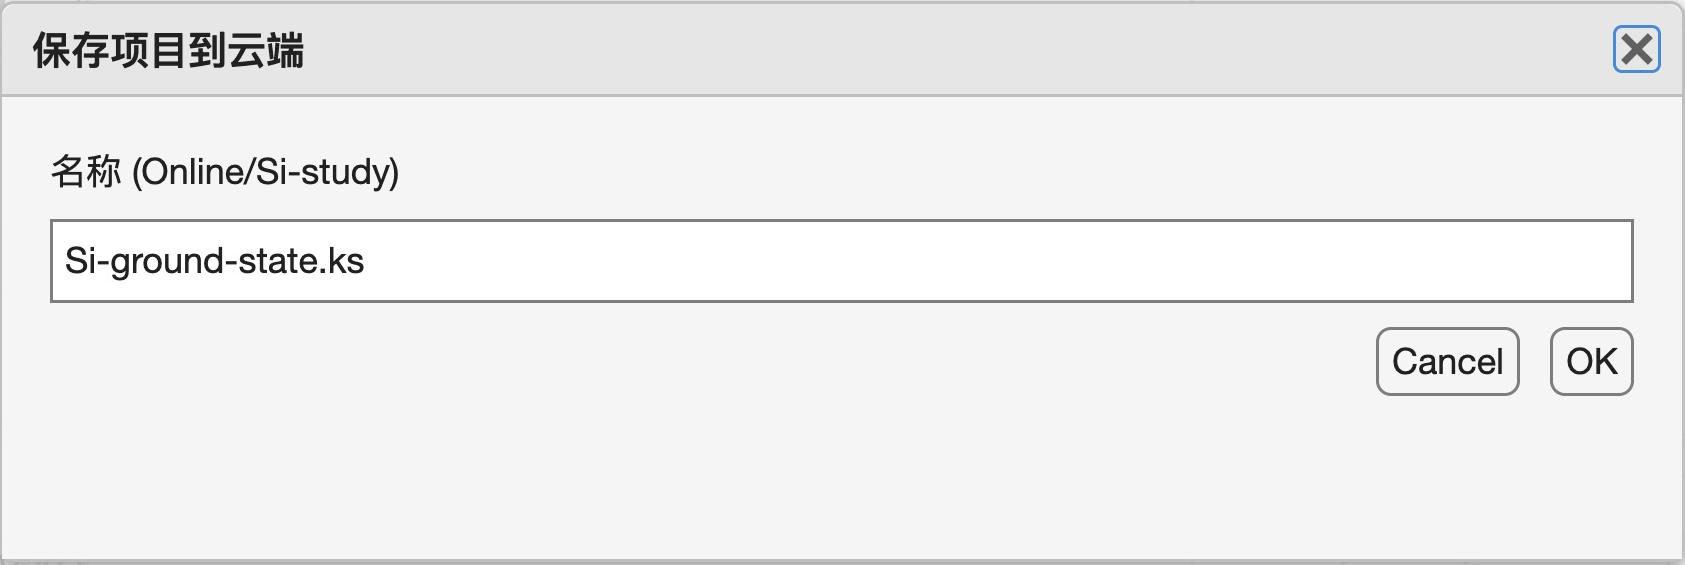
\includegraphics[width=\linewidth]{publication-assets/crop-5eed673aca0b27c69288.png}
\caption{保存项目到云端的名称窗口。名称栏填写Si-ground-state.ks，括号内显示当前选中的\file{Online/Si-study}目录。}
\label{fig:online-save-project}
\end{figure}

文件名只填写名称，不需要输入服务器完整路径。保存窗口会使用所选目录；没有填写 \file{.ks} 扩展名时，应用会补上。以后再次点击 \ui{保存}，更新的是这个项目文件。

若已经保存过项目，在文件树另选文件夹后直接保存，项目仍写回原来的位置。想要改名、保留阶段版本或放到另一目录时，应使用 \ui{另存为…}。文件面板菜单中的 \ui{保存项目到云端} 也会询问文件名，可用来把当前项目另存到所选目录。

\begin{figure}[!htb]
\centering
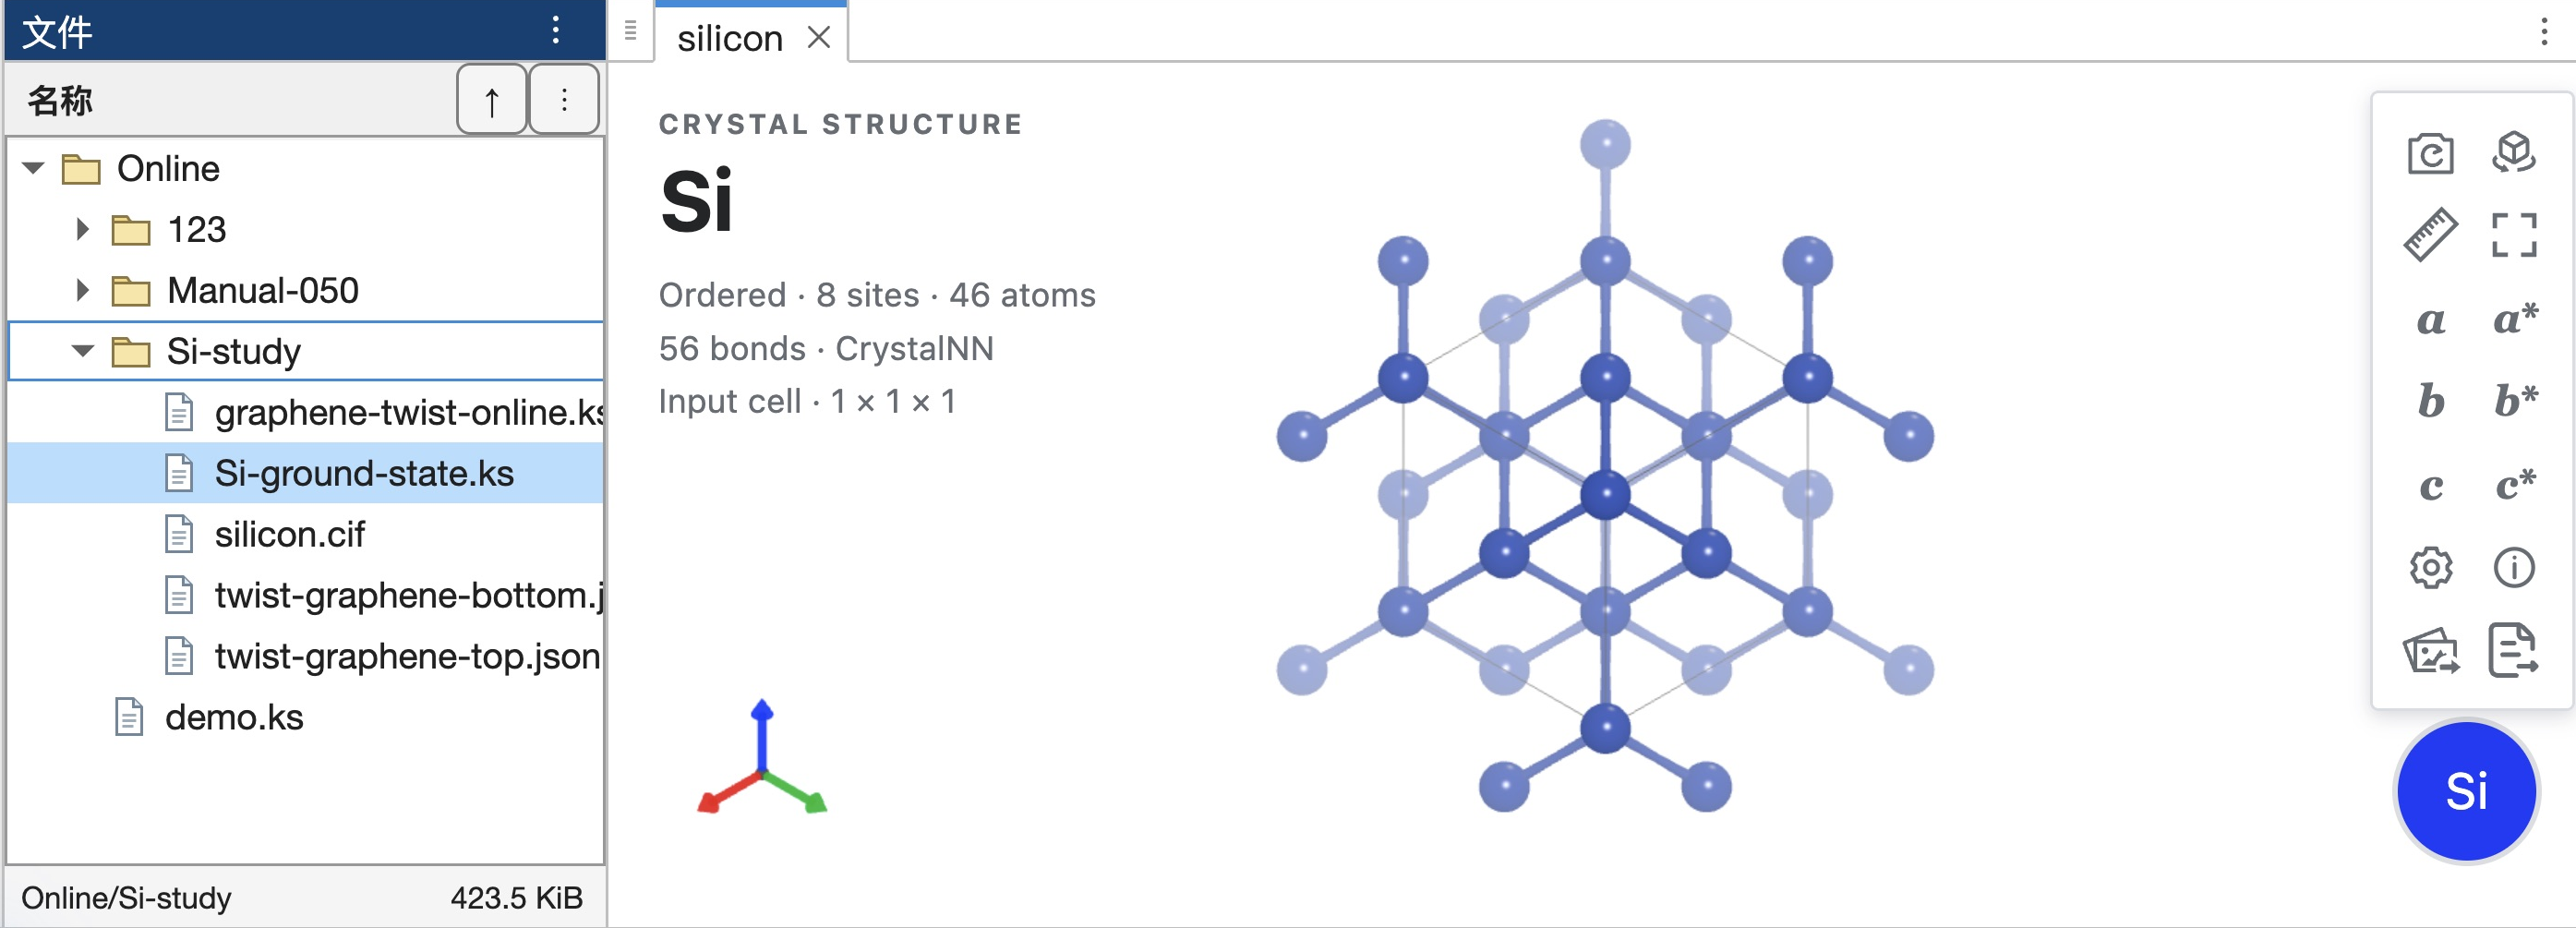
\includegraphics[width=\linewidth]{publication-assets/crop-11fbbbc4e8e9d6f1929d.png}
\caption{文件与模型的布局概览。左侧Si-study目录中选中Si-ground-state.ks，中央显示8个独立位点及包含周期映像的46个显示原子。}
\label{fig:online-workspace-silicon}
\end{figure}

图\ref{fig:online-workspace-silicon}显示文件与模型的对应关系。8 sites用于核对模型位点数，46 atoms则包含周期映像。文件名中的ground-state用于后续练习命名，不表示已经完成基态计算。

\subsection{另存一份用于比较的项目}
\index{Lingcunwei@另存为}

材料建模常需要比较不同超胞、缺陷或参数。在较大修改前保存一份阶段项目，可以让后续比较更清楚。这里先练习另存，不改变模型。

\begin{steps}
\item 在 \ui{文件} 面板选中要放置副本的目录。
\item 打开保存菜单，选择 \ui{另存为…}。
\item 输入新名称，例如 \file{Si-comparison.ks}。
\item 保存后，检查新文件已经出现，原文件仍然保留。
\end{steps}

另存后继续编辑的是新项目文件。给文件命名时可以标明材料、处理和阶段，例如“硅原胞”“硅超胞”“几何优化后”；不必把所有计算参数都塞进文件名，详细设置会留在项目中。

\section{将项目带回自己的计算机}
\index{Xiazai xiangmu@下载项目}

\subsection{下载云端文件}

云端保存便于下次登录继续工作；本机下载便于备份或与他人共享。二者可以同时使用。下载的是文件当前已经保存的内容，因此先保存，再下载。

\begin{steps}
\item 选中 \file{Si-ground-state.ks} 或刚另存的项目。
\item 从右键菜单或 \ui{⋮} 选择 \ui{下载}。
\item 等待文件准备完成。Chrome可能直接弹出本机保存窗口；选择文件夹、核对项目名后点击\ui{保存}。
\item 没有自动弹出本机窗口时，可使用页内窗口提供的\ui{Save as…}；也可以点击\mbox{\ui{Browser download}}，用浏览器的原生下载方式保存。
\item 等待浏览器下载列表显示完成；若传输窗口另有\ui{Finish}，确认本机文件已保存后再点击。
\item 在自己的文件管理器中核对项目名称和文件大小。
\end{steps}

\begin{figure}[H]
\centering
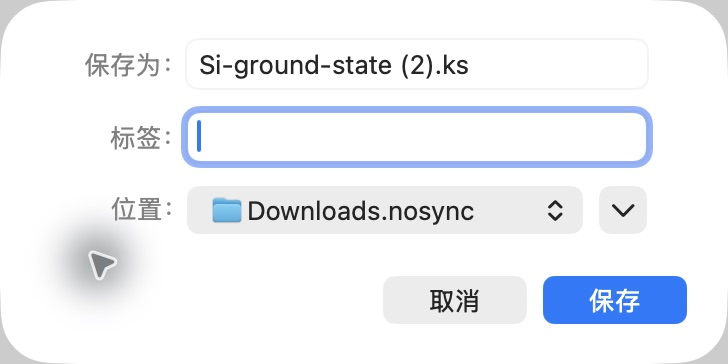
\includegraphics[width=72mm]{publication-assets/crop-348b0d07fb6f4cdab9d3.png}
\caption{macOS本机保存窗口，以随书硅项目为例。选择文件夹并核对项目名后点击保存；已有同名文件时，浏览器可能在名称后加上编号。}
\label{fig:online-project-download}
\end{figure}

浏览器设置可能让文件直接进入“下载”目录，也可能每次询问保存位置。若不知道文件去了哪里，可以打开浏览器下载列表查看。若页内窗口显示\ui{Ready to download}，表示文件已准备好交给浏览器；随后仍需完成\ui{Save as…}、\mbox{\ui{Browser download}}或下载链接对应的本机保存。本机保存后，页内准备窗口可能随之关闭。应以浏览器的完成状态和本机文件为检查点。

如果准备文件失败，窗口可能提供 \ui{Retry download}。点击后重新准备即可。取消下载不会取消云端已经完成的保存；想稍后下载时，可以重新在文件树选择同一文件。

\subsection{上传下载的大小限制}

单个上传或下载文件最多为 128~MiB；一次上传的文件总计不超过 128~MiB，最多选择 100 个。这个限制针对浏览器文件传输，并不等于账号的全部存储容量。

随着计算结果增加，项目可能明显变大。下载前可以在文件面板查看文件大小。如果超过传输上限，按部署方提供的方式处理，不要只更改扩展名或把尚未完整下载的文件用于后续处理。

本节保存并下载的结构项目随书提供为\file{examples/Si-ground-state.ks}，可用于核对硅结构和在线版文件往返操作。

\section{查看当前账号}

连接账号服务的在线版在主窗口上方显示账号名。打开账号名菜单，选择\ui{我的账号}，可进入设置中的账号页；也可以从\ui{主页 → 设置}进入该页。账号页显示当前账号名、连接状态和部署方给出的空闲释放时长。

\begin{steps}
\item 确认上方显示的是自己的账号名，打开\ui{我的账号}。
\item 查看连接状态；绿色圆点与已连接文字用于识别当前会话。空闲时长是会话策略，不是本次计算的预计完成时间。
\item 若连接需要恢复，使用账号页的\ui{重新连接}，返回工作区后检查项目与文件。
\item 结束使用前先保存项目；需要退出账号时，再使用\ui{注销}。
\end{steps}

账号页不用于修改结构和计算参数。账号名未显示或部署未提供账号页时，按入口页提供的连接方式返回工作区。


\section{离开工作空间}

\subsection{临时返回入口}

账号菜单中的 \ui{退出 KSSOLV Toolbox} 会返回入口，工作空间继续保留至空闲超时。保留当前浏览器标签页时，入口中的 \ui{重连工作空间} 可以回到原界面，适合暂时查看入口状态后继续工作。

这一操作与注销不同。暂时返回入口并不会立即释放计算资源，也不会把项目自动保存到磁盘。重要修改仍应先保存。

可以用本章的氢分子项目练习一次返回与重连：
\begin{steps}
\item 保存当前项目，确认计算已经结束。
\item 打开上方账号菜单，选择\ui{退出 KSSOLV Toolbox}。阅读保留工作空间的提示，确认后返回入口。
\item 核对入口显示\ui{已返回入口，工作空间仍在运行}，再点击\ui{重连工作空间}。
\item 回到工作区后检查原项目：SCF流程仍有Configuration、SCF与Plot三个节点，Results中的Run SCF数据集和EnergyConvergence曲线仍在。打开曲线，确认可以继续阅读结果。
\end{steps}

\begin{figure}[!htb]
\centering
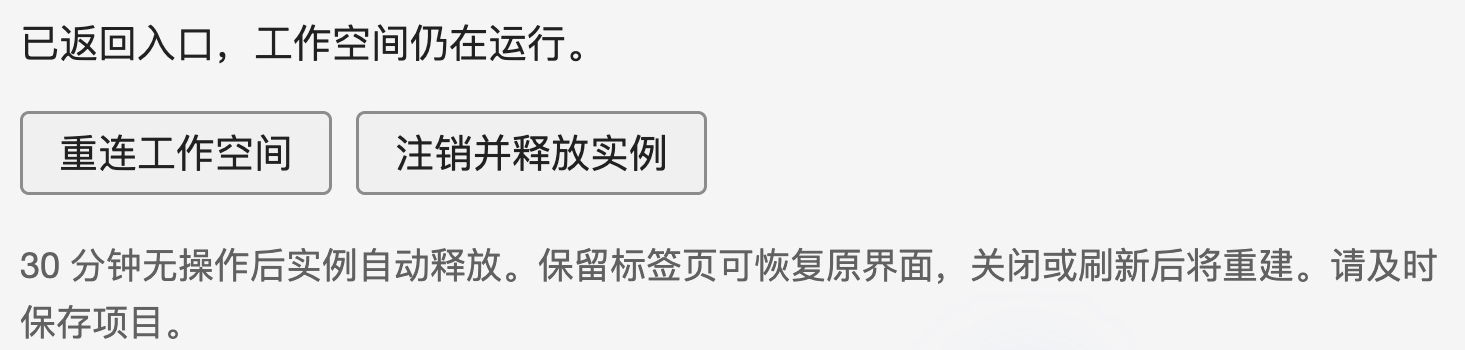
\includegraphics[width=122mm]{publication-assets/crop-432edbee8ecb03b7c537.png}
\caption{正常返回入口后的状态与重连按钮。本次通过\ui{重连工作空间}回到原氢分子项目；\ui{注销并释放实例}是另一个操作。空闲时长以当前部署提示为准。}
\label{fig:online-reconnect}
\end{figure}

\subsection{关闭或刷新网页}
\index{Chonglian@重新连接}

关闭网页不等于注销。重新访问同一固定入口时，如果原工作空间仍然存活，可以重新连接，并重新建立浏览器界面。项目、已打开的结构与工作流等内容可以在同一运行实例中恢复；但临时对话框、撤销历史和完整布局不必然保持原样。

刷新页面也会重建浏览器界面，因此不要把刷新当作普通的保存或恢复命令。网络短暂中断时，先等连接恢复，或从固定入口重连；需要保留当前布局时，使用入口返回而非反复刷新。

\subsection{注销并释放工作空间}

结束今天的工作，尤其是在共享计算机上，先保存项目，再从账号菜单选择 \ui{注销}，或在入口点击 \ui{注销并释放实例}。确认后会结束访问会话并释放运行实例。

下一次登录会使用同一账号的云端文件。此前保存的项目和设置仍然保留，但仅在内存中的变量、未保存修改和运行中的计算不能依靠注销后恢复。因此，离开前最有用的检查是：项目已保存，必要的结果已经取回，重要文件已经下载。

% SCREENSHOT: 已补正常返回入口后的状态、重连按钮与保存提示，见fig:online-reconnect；不另重复账号菜单图。

\subsection{理解空闲释放}

在线版的空闲释放时间由平台设定，当前值可以在账号设置或入口提示中查看。不同部署可能采用不同的时长，接近释放时页面会显示提醒。键盘、点击、触摸和滚动表示存在交互操作；仅将标签页留在前台，或让状态自动刷新，并不延长空闲时间。

计算正在运行也不表示始终存在交互操作。安排较长任务前，应了解平台对空闲释放和长时计算的安排。需要使用独立集群队列时，按照所用集群的使用说明操作；完整 MATLAB\regmark{} 工具箱的远程提交见第~\ref{ch:remote}~章。小型入门练习则适合在仍能观察结果的时间内完成。

\Needspace{6\baselineskip}
\begin{notebox}{确认文件确实保留}
完成本章练习后，保存项目并注销。再次登录，在“文件”面板找到练习目录，双击保存的 \file{.ks}，检查结构是否仍在。这个检查有助于确认云端文件的保存与重新打开过程。
\end{notebox}

\section{处理工作空间连接}

工作区底部的资源状态用于了解当前运行环境的 CPU 和内存占用。在按账号分配资源的部署中，它反映分配给当前工作区的资源；普通容器部署也可能显示宿主机环境。具体含义以状态栏标识与部署说明为准，不应直接把“CPU 使用率高”理解为计算错误。

工作流的资源选项取决于节点任务、求解方法和部署所支持的计算环境。配置时先选中目标节点，再查看其资源面板；具体选择与检查方法见第\ref{sec:node-resources}节。主页的\ui{并行}按钮不代替节点资源设置，服务器是否具备进程池或GPU支持也需按部署条件确认。

熟悉文件操作后，可以继续第~\ref{ch:first}~章的氢分子计算。先把随书\file{h2.cif}上传到自己的云端目录，再导入当前项目。随后建立SCF工作流，按该章填写结构输入和求解参数。

图\ref{fig:online-h2-config}展示了本次在线版练习采用的结构输入设置。选中节点后，使用\ui{工作流 → 配置节点}，向下查看\ui{选项}。本例的结构配置节点标为\ui{Configuration}，对应\ui{Build Molecule}任务；选择Molecule、结构h2、PBE、default赝势、20 Ha、0 K与Nspin=1。SCF节点的求解方法和最大步数仍按第~\ref{ch:first}~章设置。

\begin{figure}[!htb]
\centering
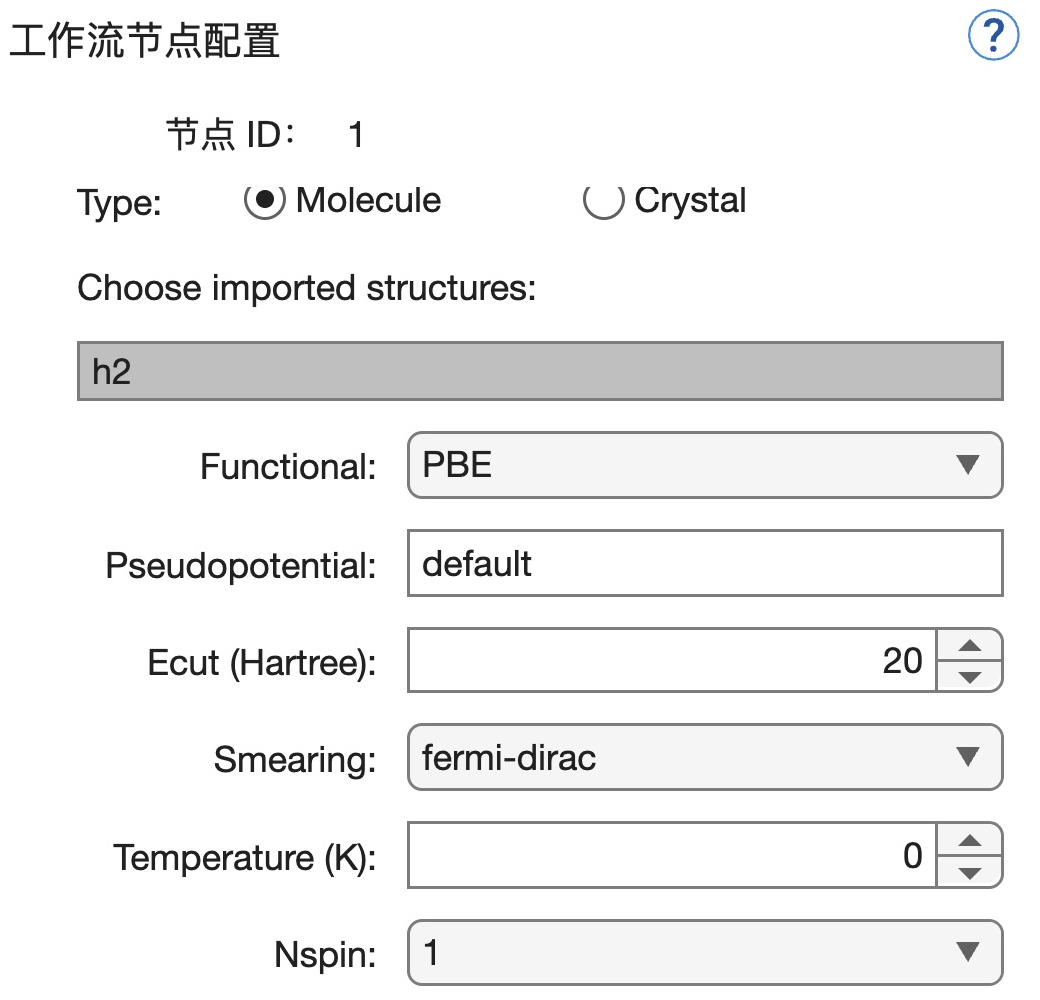
\includegraphics[width=88mm]{publication-assets/crop-434fe0ac4d3f46cfaf46.png}
\caption{氢分子工作流的结构输入选项。所选h2结构和计算条件都在右侧配置编辑器中核对。}
\label{fig:online-h2-config}
\end{figure}

本次在线版计算在7步达到收敛，日志与参考运行的比较见第~\ref{ch:first}~章。计算结束后，点击项目浏览器侧边按钮，展开\ui{Results}：\ui{Datasets}下的\ui{Run SCF}保存这次运行的数据，\ui{Plots}下的\ui{EnergyConvergence}打开收敛图。

检查日志和曲线后，再次保存项目，关闭当前项目，然后从\ui{文件}面板双击保存的\file{.ks}重新打开。图\ref{fig:online-h2-results}是本次保存后重新打开的项目树：数据集与曲线仍在各自分组中。再次双击\ui{EnergyConvergence}，可以读到刚才七次迭代的收敛图。最后从云端下载项目，保留本机副本。

\begin{figure}[!htb]
\centering
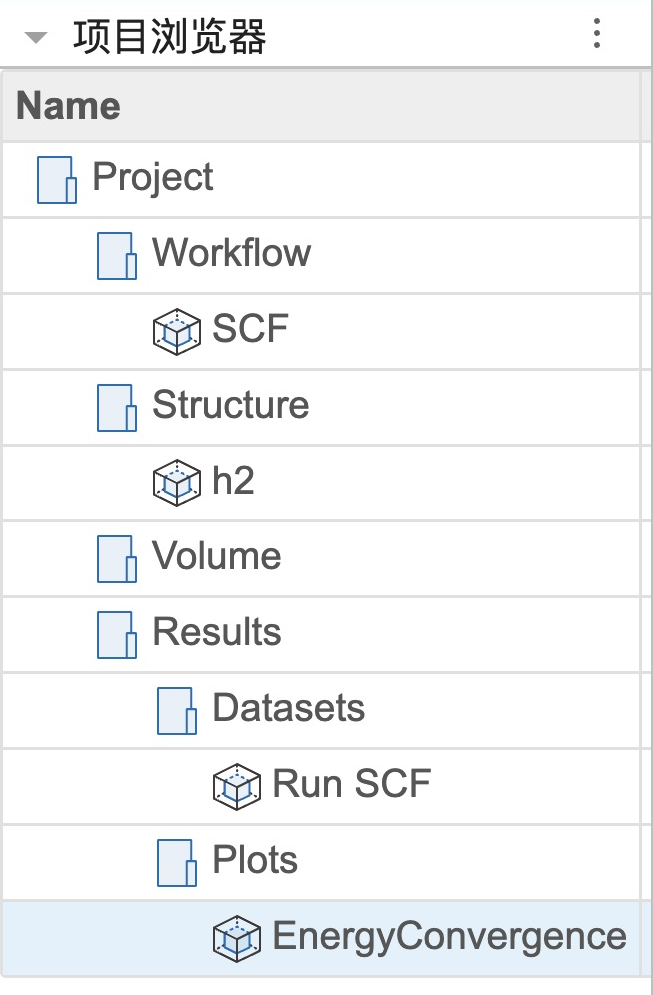
\includegraphics[width=55mm]{publication-assets/crop-c36a9eee3be02622a4d7.png}
\caption{保存后重新打开的氢分子项目。Results保留本次计算的Run SCF数据集与EnergyConvergence收敛图；双击曲线条目可以继续查看七次迭代的结果。}
\label{fig:online-h2-results}
\end{figure}

这样，结构准备、服务器计算、保存与重新打开就连成了一次完整练习。

连接失败时先回固定入口，查看工作空间是否仍在启动。如果入口显示 \ui{重试连接}，先使用此操作。持续不可用时，入口可能提供 \ui{重启工作空间}；重启保留已保存文件和设置，但结束当前内存会话，确认后再操作。

忘记密码时，在登录页点击 \ui{忘记密码}，先取得个人备忘问题，再填写答案和新密码。重置过程会结束已有会话，成功后重新登录；若没有设置问题或忘记答案，请联系管理员。

\section{没有云端文件面板的浏览器会话}

界面若提示“当前部署未启用持久化文件”，打开文件需从本机上传，保存时通过浏览器下载。离开前确认本机已有副本。
